\mode<presentation>
{
  \usetheme{CambridgeUS}
  \usecolortheme{whale}
  \usecolortheme{lily}

  \setbeamercovered{transparent}
  \usefonttheme[onlymath]{serif}
}

\title[\BlockDiagramsShortName] 
{\course: \BlockDiagramsName\license}

\subtitle{Lecture \BlockDiagramsNumber}

\begin{document}

\begin{frame}
  \titlepage
\end{frame}

\mode<article>{
\maketitle
\tableofcontents
}


\section{Pre-requisite Material}
This lecture assumes that the reader is familiar with the following material:
\begin{itemize}
\item Lecture \ImpedanceNumber:~\ImpedanceName
\end{itemize}

\section{Block Diagrams as Control Systems Tools}

When working with complicated systems, it can be useful to break the system up into smaller interconnected subsystems. This is useful both as a modeling technique as well as to gain insight into the operation of a system. 

Block diagrams are a graphical tool that we use to visually represent the algebraic equations that are needed to model interconnected subsystems. In this lecture, we'll start to be more precise with the building blocks of Laplace-domain modeling for physical systems than we have been so far. In particular, we'll formalize block diagrams as pictorial representations of algebra consisting of (1) signals and (2) the relationships between them. 


\subsection{Block Diagram Elements}



There are three basic elements of a block diagram: signals (arrows), systems, and summing junctions (sometimes called ``summers''). 

\begin{frame}{Block Diagram Elements}
\begin{center}
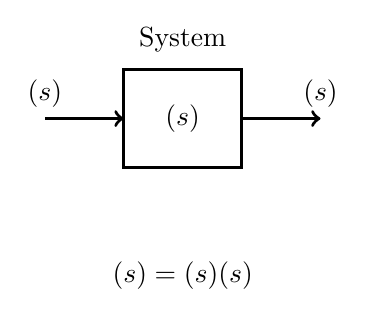
\begin{tikzpicture}[inner sep=0pt,outer sep=0pt,very thick,
sysblock/.style={draw,rectangle,inner sep=2pt,minimum width=1.5cm,minimum height=1.25cm,very thick}]
%\draw (0,0) node[draw,circle] (sum) {$\rule{0pt}{18pt}$};
\draw (0,0) node[sysblock] (G) {$\plant(s)$};
\draw[<-] (G.180) -- ++(-1,0) node[above=4pt] {$\inptLT(s)$};
\draw[->] (G.0) -- ++(1,0) node[above=4pt] {$\outptLT(s)$};
\draw (0,-2) node {$\outptLT(s)=\plant(s)\inptLT(s)$};
\draw (0,1) node {System};
\end{tikzpicture}
\hspace{0.5in}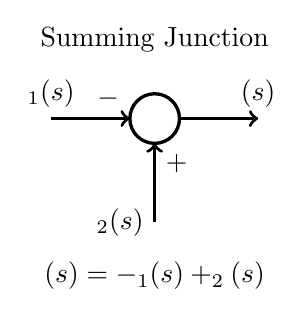
\begin{tikzpicture}[inner sep=0pt,outer sep=0pt,very thick,
sysblock/.style={draw,rectangle,inner sep=2pt,minimum width=1.5cm,minimum height=1.25cm,very thick}]
\draw (0,0) node[draw,circle] (sum) {$\rule{0pt}{18pt}$};
\draw[<-] (sum.180) node[above left=4pt] {$-$} -- ++(-1,0) node[above=4pt] {$\inptLT_{1}(s)$};
\draw[<-] (sum.-90) node[below right=4pt] {$+$} -- ++(0,-1) node[left=4pt] {$\inptLT_{2}(s)$};
\draw[->] (sum.0) -- ++(1,0) node[above=4pt] {$\outptLT(s)$};
\draw (0,-2) node {$\outptLT(s)=-\inptLT_{1}(s)+\inptLT_{2}(s)$};
\draw (0,1) node {Summing Junction};
\end{tikzpicture}

\end{center}
\end{frame}

As shown in these images, both systems and summing junctions represent algebraic relationships, namely multiplication and addition. In particular, a Laplace-domain output signal $Y(s)$ can be found by multiplying the input signal $R(s)$ by the plant's transfer function $G(s)$.

\subsection{Block Diagram Simplifications}

Systems and summing junctions can be combined in many different ways. A basic modeling tool will be to simplify a block diagram to determine the equivalent transfer function that represents the overall system. 
Some of the most common simplifications are combining systems in series, parallel, and feedback. 

Systems that are in series (or cascade) can be combined into a single system by multiplying the system transfer functions. 
\begin{frame}{Block Diagram Simplifications:}{Systems in Series}
\begin{center}
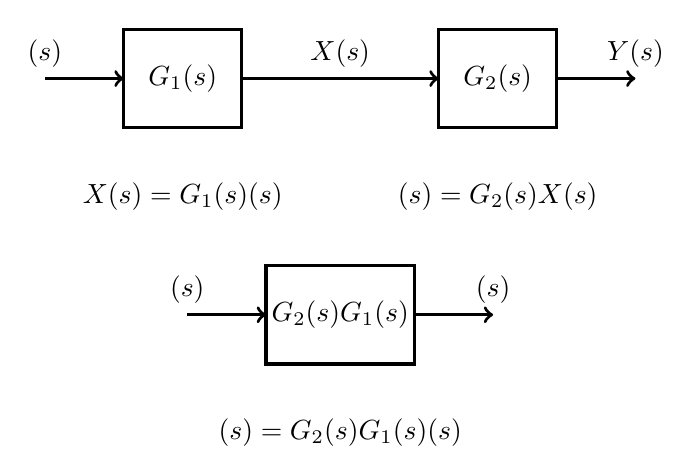
\begin{tikzpicture}[inner sep=0pt,outer sep=0pt,very thick,
sysblock/.style={draw,rectangle,inner sep=2pt,minimum width=1.5cm,minimum height=1.25cm,very thick}]
%\draw (0,0) node[draw,circle] (sum) {$\rule{0pt}{18pt}$};
\draw (0,0) node[sysblock] (G1) {$G_{1}(s)$};
\draw (4,0) node[sysblock] (G2) {$G_{2}(s)$};
\draw[<-] (G1.180) -- ++(-1,0) node[above=4pt] {$\inptLT(s)$};
\draw[->] (G1.0) -- node[pos=.5,above=4pt] {$X(s)$} (G2.180);
\draw[->] (G2.0) -- ++(1,0) node[above=4pt] {$Y(s)$};
\draw (0,-1.5) node {$X(s)=G_{1}(s)\inptLT(s)$};
\draw (4,-1.5) node {$\outptLT(s)=G_{2}(s)X(s)$};

\draw (2,-3) node[sysblock] (GG) {$G_{2}(s)G_{1}(s)$};
\draw[<-] (GG.180) -- ++(-1,0) node[above=4pt] {$\inptLT(s)$};
\draw[->] (GG.0) -- ++(1,0) node[above=4pt] {$\outptLT(s)$};
\draw (2,-4.5) node {$\boxed{\outptLT(s)=G_{2}(s)G_{1}(s)\inptLT(s)}$};

\end{tikzpicture}

\end{center}
\end{frame}

Notice that these systems may appear visually to be similar to impedances in series within an impedance network, but they are not! In the ``series'' example, two impedances would be combined by adding them, whereas for block diagrams the algebra shows us that systems are combined by multiplication. It may help to think of an impedance network as a circuit (even if it's representing a mechanical or other type of system) and a block diagram as an algebraic equation. 

Again, by noting the algebraic relationships represented, systems in parallel can be combined by adding
\begin{frame}{Block Diagram Simplifications:}{Systems in Parallel}
\begin{center}
\mode<presentation>{\resizebox{5cm}{!}{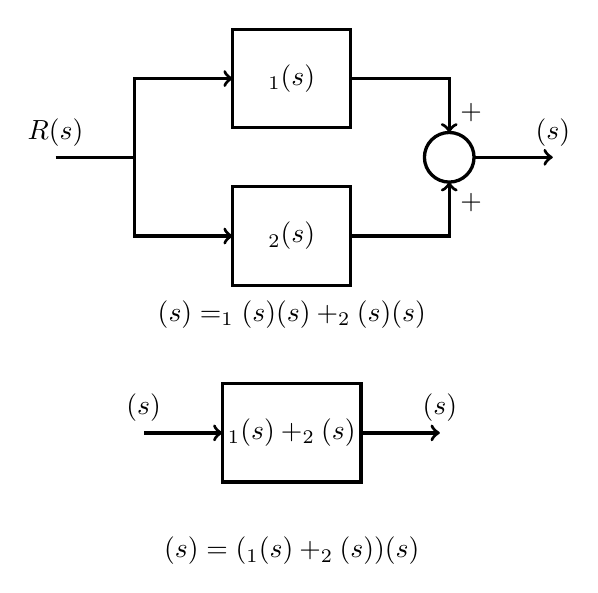
\begin{tikzpicture}[inner sep=0pt,outer sep=0pt,very thick,
sysblock/.style={draw,rectangle,inner sep=2pt,minimum width=1.5cm,minimum height=1.25cm,very thick}]
\draw (1,1) node[sysblock] (G1) {$\plant_{1}(s)$};
\draw (1,-1) node[sysblock] (G2) {$\plant_{2}(s)$};
\draw (-2,0) node[above=4pt] {$R(s)$} -- (-1,0);
\draw[->] (-1,0) |- (G1.180);
\draw[->] (-1,0) |- (G2.180);
\draw (3,0) node[draw,circle] (sum) {$\rule{0pt}{18pt}$};
\draw[->] (G1.0) -| (sum.90) node[above right=4pt] {$+$};
\draw[->] (G2.0) -| (sum.-90) node[below right=4pt] {$+$};
\draw[->] (sum.0) -- ++(1,0) node[above=4pt] {$\outptLT(s)$};
\draw (1,-2) node {$\outptLT(s)=\plant_{1}(s)\inptLT(s) + \plant_{2}(s)\inptLT(s)$};

\draw (1,-3.5) node[sysblock] (GG) {$\plant_{1}(s)+\plant_{2}(s)$};
\draw[<-] (GG.180) -- ++(-1,0) node[above=4pt] {$\inptLT(s)$};
\draw[->] (GG.0) -- ++(1,0) node[above=4pt] {$\outptLT(s)$};
\draw (1,-5) node {$\boxed{\outptLT(s)=(\plant_{1}(s)+\plant_{2}(s))\inptLT(s)}$};

\end{tikzpicture}
}}
\mode<article>{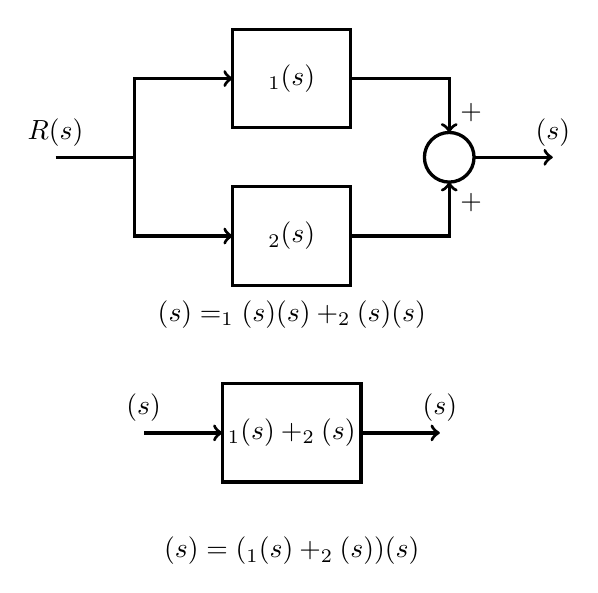
\begin{tikzpicture}[inner sep=0pt,outer sep=0pt,very thick,
sysblock/.style={draw,rectangle,inner sep=2pt,minimum width=1.5cm,minimum height=1.25cm,very thick}]
\draw (1,1) node[sysblock] (G1) {$\plant_{1}(s)$};
\draw (1,-1) node[sysblock] (G2) {$\plant_{2}(s)$};
\draw (-2,0) node[above=4pt] {$R(s)$} -- (-1,0);
\draw[->] (-1,0) |- (G1.180);
\draw[->] (-1,0) |- (G2.180);
\draw (3,0) node[draw,circle] (sum) {$\rule{0pt}{18pt}$};
\draw[->] (G1.0) -| (sum.90) node[above right=4pt] {$+$};
\draw[->] (G2.0) -| (sum.-90) node[below right=4pt] {$+$};
\draw[->] (sum.0) -- ++(1,0) node[above=4pt] {$\outptLT(s)$};
\draw (1,-2) node {$\outptLT(s)=\plant_{1}(s)\inptLT(s) + \plant_{2}(s)\inptLT(s)$};

\draw (1,-3.5) node[sysblock] (GG) {$\plant_{1}(s)+\plant_{2}(s)$};
\draw[<-] (GG.180) -- ++(-1,0) node[above=4pt] {$\inptLT(s)$};
\draw[->] (GG.0) -- ++(1,0) node[above=4pt] {$\outptLT(s)$};
\draw (1,-5) node {$\boxed{\outptLT(s)=(\plant_{1}(s)+\plant_{2}(s))\inptLT(s)}$};

\end{tikzpicture}
}
\end{center}
\end{frame}

Both the series and parallel combinations shown so far are \textit{open loop}; that is, there are no signals (arrows) from which we can sketch a path, following the arrow directionality, and return to the original arrow. The next configuration that we will review is a \textit{closed loop} combination, otherwise known as a feedback connection. 
%The following is a basic feedback connection. 
Note that the output $Y(s)$ of the system $G(s)$ appears at the input of the other system, $H(s)$. To derive the equivalent single system, we first write the equations represented by this block diagram.
\begin{frame}{Block Diagram Simplifications:}{Systems in Feedback}
\begin{center}
\begin{tikzpicture}[inner sep=0pt,outer sep=0pt,very thick,
sysblock/.style={draw,rectangle,inner sep=2pt,minimum width=1.5cm,minimum height=1.25cm,very thick}]
\draw (-1,0) node[draw,circle] (sum) {$\rule{0pt}{18pt}$};
\draw (1,0) node[sysblock] (G1) {$\plant(s)$};
\draw (1,-2) node[sysblock] (G2) {$H(s)$};
\draw (-2.5,0) node[above=4pt] {$\inptLT(s)$} -- (sum.180) node[above left=4pt] {$+$};
\draw[->] (sum.0) -- node[pos=.5,above=4pt] {$E(s)$} (G1.180);
\draw[->] (G1.0) -- ++(1,0) |- (G2.0);
\draw[->] (G2.180) -| (sum.-90) node[below right] {$-$};
\draw[->] (G1.0) -- ++(2,0) node[above=4pt] {$\outptLT(s)$};
\draw (1,-3.5) node {$\begin{aligned}\outptLT(s)&=\plant(s)E(s)\\E(s) &= \inptLT(s) - H(s)\outptLT(s)\end{aligned}$};


\end{tikzpicture}

\end{center}
\end{frame}
From these two equations, since we are interested in the relationship from the overall input $R(s)$ to the overall output $Y(s)$, we can eliminate the intermediate variable $E(s)$ to derive the simplified system relationship.
\begin{align*}
\outptLT(s) &= \plant(s)\left(\inptLT(s) - H(s)\outptLT(s)\right) \\
& = \plant(s)\inptLT(s)  - \plant(s)H(s)\outptLT(s)
\end{align*}
Thus, solving for $\outptLT(s)$:
\begin{align*}
\outptLT(s) + \plant(s)H(s)\outptLT(s) &= \plant(s)\inptLT(s)\\
(1+\plant(s)H(s))\outptLT(s) & = \plant(s) \inptLT(s) \\
\outptLT(s) & = \frac{\plant(s)}{1+\plant(s)H(s)}\inptLT(s)
\end{align*}
We will use this simplification often in this course.
\begin{frame}{Block Diagram Simplifications:}{Feedback Simplification}
\[
\boxed{\outptLT(s) = \frac{\plant(s)}{1+\plant(s)H(s)}\inptLT(s)}
\]
\begin{center}
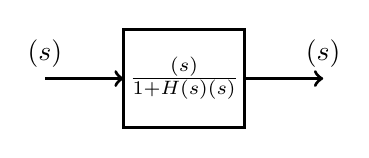
\begin{tikzpicture}[inner sep=0pt,outer sep=0pt,very thick,
sysblock/.style={draw,rectangle,inner sep=2pt,minimum width=1.5cm,minimum height=1.25cm,very thick}]
\draw (0,0) node[sysblock] (G1) {$\frac{\plant(s)}{1+H(s)\plant(s)}$};
\draw[<-] (G1.180) -- ++(-1,0) node[above=4pt] {$\inptLT(s)$};
\draw[->] (G1.0) -- ++(1,0) node[above=4pt] {$\outptLT(s)$};
\end{tikzpicture}

\end{center}
\end{frame}

\subsection{Example}

\begin{frame}{Example 1}
\begin{itemize}
\item Simplify the following block diagram. All variables are functions of s.
\end{itemize}
\begin{center}
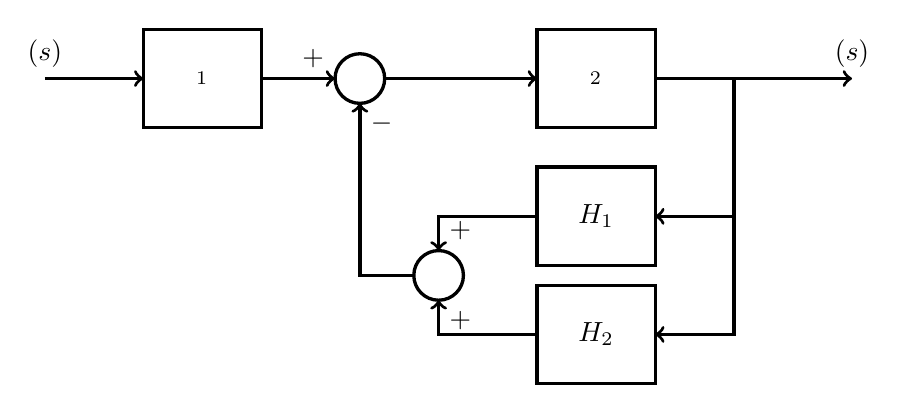
\begin{tikzpicture}[inner sep=0pt,outer sep=0pt,very thick,
sysblock/.style={draw,rectangle,inner sep=2pt,minimum width=1.5cm,minimum height=1.25cm,very thick}]
\draw (0,0) node[sysblock] (G1) {$\plant_{1}$};
\draw (2,0) node[draw,circle] (sum1) {$\rule{0pt}{18pt}$};
\draw (5,0) node[sysblock] (G2) {$\plant_{2}$};
\draw (G2.0) ++(1,0) node[fill=black] (a) {};

\draw (5,-1.75) node[sysblock] (H1) {$H_{1}$};
\draw (5,-3.25) node[sysblock] (H2) {$H_{2}$};
\draw (3,-2.5) node[draw,circle] (sum2) {$\rule{0pt}{18pt}$};

\draw[->] (-2,0) node[above=4pt] {$\inptLT(s)$} -- (G1.180);
\draw[->] (G1.0) -- (sum1.180) node[above left=4pt] {$+$};
\draw[->] (sum1.0) -- (G2.180);
\draw (G2.0) -- (a);
\draw[->] (a) -- ++(1.5,0) node[above=4pt] {$\outptLT(s)$};
\draw[->] (a) |- (H1.0);
\draw[->] (a) |- (H2.0);
\draw[->] (H1.180) -| (sum2.90) node[above right=4pt] {$+$};
\draw[->] (H2.180) -| (sum2.-90) node[below right=4pt] {$+$};
\draw[->] (sum2.180) -| (sum1.-90) node[below right=4pt] {$-$};

\end{tikzpicture}

\end{center}
\end{frame}

\begin{frame}{Example 1:}{Step 1}
\begin{itemize}
\item Combine systems in parallel
\end{itemize}
\begin{center}
\input{figures/blockdiagramexample1simp1.tex}
\end{center}
\end{frame}

\begin{frame}{Example 1:}{Steps 2 and 3}
\begin{itemize}
\item Combine feedback systems
\item Combine systems in series
\end{itemize}
\begin{center}
\begin{tikzpicture}[inner sep=0pt,outer sep=0pt,very thick,
sysblock/.style={draw,rectangle,inner sep=2pt,minimum width=1.5cm,minimum height=1.25cm,very thick}]
\draw (0,0) node[sysblock] (G1) {$\plant_{1}$};
\draw (-2,0) node[above=4pt] {$\inptLT(s)$} -- (G1.180);
\draw (4,0) node[sysblock] (G2) {$\frac{G_{2}}{1+(H_{1}+H_{2})G_{2}}$};
\draw (G2.0) ++(1,0) node[fill=black] (a) {};

\draw[->] (G1.0) -- (G2.180);
\draw (G2.0) -- (a);
\draw[->] (a) -- ++(1,0) node[above=4pt] {$\outptLT(s)$};


\draw (2,-2) node[sysblock] (G) {$\frac{\plant_{2}\plant_{1}}{1+(H_{1}+H_{2})\plant_{2}}$};
\draw[<-] (G.180) -- ++(-1,0) node[above=4pt] {$\inptLT(s)$};
\draw[->] (G.0) -- ++(1,0) node[above=4pt] {$\outptLT(s)$};
\end{tikzpicture}

\end{center}
\end{frame}

\subsection{Moving Elements}

\begin{frame}{Moving Summers}
\begin{itemize}
\item Since addition is commutative, summing can be done in any order
\end{itemize}
\begin{center}
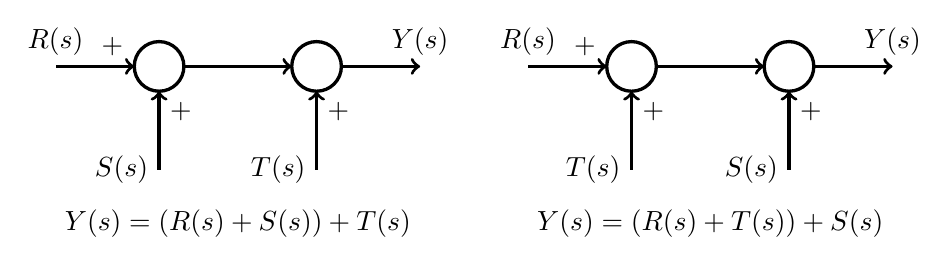
\begin{tikzpicture}[inner sep=0pt,outer sep=0pt,very thick,
sysblock/.style={draw,rectangle,inner sep=2pt,minimum width=1.5cm,minimum height=1.25cm,very thick}]
\draw (0,0) node[draw,circle] (sum) {$\rule{0pt}{18pt}$};
\draw (2,0) node[draw,circle] (sum2) {$\rule{0pt}{18pt}$};
\draw[<-] (sum.180) node[above left=4pt] {$+$} -- ++(-1,0) node[above=4pt] {$R(s)$};
\draw[<-] (sum.-90) node[below right=4pt] {$+$} -- ++(0,-1) node[left=4pt] {$S(s)$};
\draw[->] (sum.0) -- (sum2.180);
\draw[<-] (sum2.-90) node[below right=4pt] {$+$} -- ++(0,-1) node[left=4pt] {$T(s)$};
\draw[->] (sum2.0) -- ++(1,0) node[above=4pt] {$Y(s)$};
\draw (1,-2) node {$Y(s)=\left(R(s)+S(s)\right)+T(s)$};

\draw (6,0) node[draw,circle] (sum) {$\rule{0pt}{18pt}$};
\draw (8,0) node[draw,circle] (sum2) {$\rule{0pt}{18pt}$};
\draw[<-] (sum.180) node[above left=4pt] {$+$} -- ++(-1,0) node[above=4pt] {$R(s)$};
\draw[<-] (sum.-90) node[below right=4pt] {$+$} -- ++(0,-1) node[left=4pt] {$T(s)$};
\draw[->] (sum.0) -- (sum2.180);
\draw[<-] (sum2.-90) node[below right=4pt] {$+$} -- ++(0,-1) node[left=4pt] {$S(s)$};
\draw[->] (sum2.0) -- ++(1,0) node[above=4pt] {$Y(s)$};
\draw (7,-2) node {$Y(s)=\left(R(s)+T(s)\right)+S(s)$};

\end{tikzpicture}

\end{center}
\end{frame}

\begin{frame}{Moving Pick-off points}
\begin{itemize}
\item Pick-off points can be taken anywhere on a line
\end{itemize}
\begin{center}
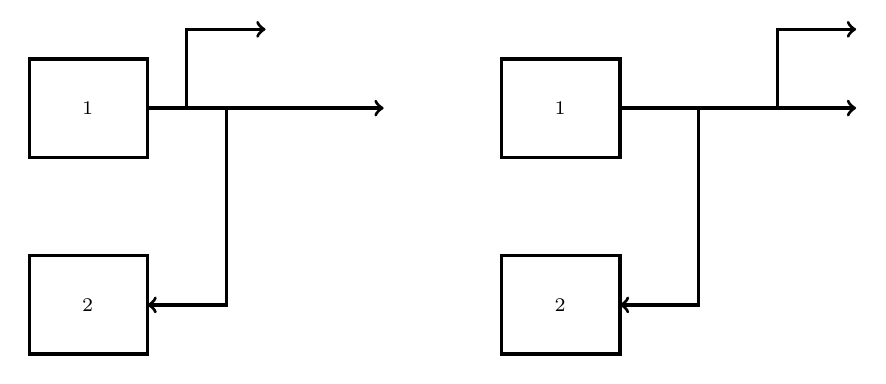
\begin{tikzpicture}[inner sep=0pt,outer sep=0pt,very thick,
sysblock/.style={draw,rectangle,inner sep=2pt,minimum width=1.5cm,minimum height=1.25cm,very thick}]

\draw (0,0) node[sysblock] (G1) {$\plant_{1}$};
\draw (0,-2.5) node[sysblock] (G2) {$\plant_{2}$};
\draw[->] (G1.0) -- ++(3,0);
\draw[->] (G1.0) ++(1,0) |- (G2.0);
\draw[->] (G1.0) ++(.5,0) -- ++(0,1) -- ++(1,0);


\draw (6,0) node[sysblock] (G1) {$\plant_{1}$};
\draw (6,-2.5) node[sysblock] (G2) {$\plant_{2}$};
\draw[->] (G1.0) -- ++(3,0);
\draw[->] (G1.0) ++(1,0) |- (G2.0);
\draw[->] (G1.0) ++(2,0) -- ++(0,1) -- ++(1,0);

\end{tikzpicture}

\end{center}
\end{frame}

\begin{frame}{Moving Pick-off points around blocks}
\begin{itemize}
\item Pick-off points can be moved around a block by adding blocks
\end{itemize}
\begin{center}
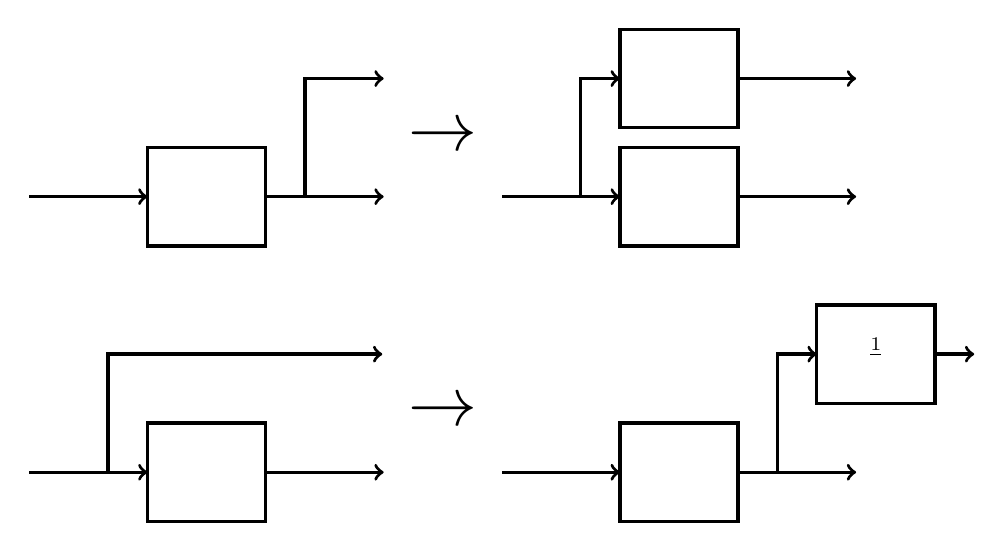
\begin{tikzpicture}[inner sep=0pt,outer sep=0pt,very thick,
sysblock/.style={draw,rectangle,inner sep=2pt,minimum width=1.5cm,minimum height=1.25cm,very thick}]

\draw (0,0) node[sysblock] (G1) {$\plant$};
\draw[<-] (G1.180) -- ++(-1.5,0);
\draw[->] (G1.0) -- ++(1.5,0);
\draw[->] (G1.0) ++(.5,0) -- ++(0,1.5) -- ++(1,0);

\draw (3,.75) node {\Huge $\rightarrow$};

\draw (6,0) node[sysblock] (G1) {$\plant$};
\draw (6,1.5) node[sysblock] (G2) {$\plant$};
\draw[<-] (G1.180) -- ++(-1.5,0);
\draw[->] (G1.0) -- ++(1.5,0);
\draw[->] (G1.180) ++(-.5,0) |- (G2.180);
\draw[->] (G2.0) -- ++(1.5,0);


\draw (0,-3.5) node[sysblock] (G3) {$\plant$};
\draw (G3.0) ++(1.5,1.5) node (a) {};
\draw[<-] (G3.180) -- ++(-1.5,0);
\draw[->] (G3.0) -- ++(1.5,0);
\draw[->] (G3.180) ++(-.5,0) |- (a);

\draw (3,-2.75) node {\Huge $\rightarrow$};


\draw (6,-3.5) node[sysblock] (G3) {$\plant$};
\draw (8.5,-2) node[sysblock] (G4) {$\frac{1}{\plant}$};
\draw (G3.0) ++(2,1.5) node (a) {};
\draw[<-] (G3.180) -- ++(-1.5,0);
\draw[->] (G3.0) -- ++(1.5,0);
\draw[->] (G3.0) ++(0.5,0) |- (G4);
\draw[->] (G4.0) -- ++(.5,0);

\end{tikzpicture}

\end{center}
\end{frame}

\subsection{Simplifying a Block Diagram with Algebra}
\begin{frame}{Backup Plan}
If you ever get stuck - just convert back to algebra relationships and solve these by hand
\begin{enumerate}
\item First, add signal names at inputs to blocks (pick any unused letter)
\item Then, write equations for all variables
\item Finally, eliminate the intermediate variables (signals you labeled, not the primary input and output signals) and solve for transfer function
\end{enumerate}
\begin{center}
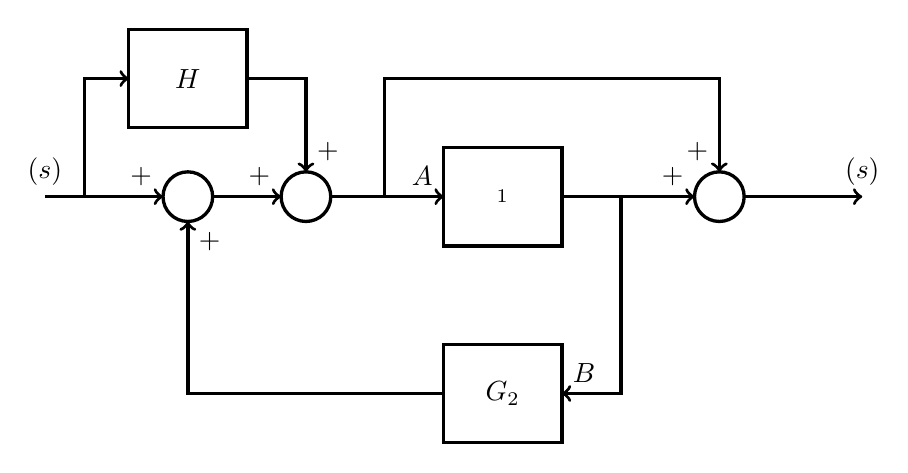
\begin{tikzpicture}[inner sep=0pt,outer sep=0pt,very thick,
sysblock/.style={draw,rectangle,inner sep=2pt,minimum width=1.5cm,minimum height=1.25cm,very thick}]
\draw (1,0) node[draw,circle] (sum1) {$\rule{0pt}{18pt}$};
\draw (2.5,0) node[draw,circle] (sum3) {$\rule{0pt}{18pt}$};
\draw (1,1.5) node[sysblock] (H) {$H$};
\draw (5,0) node[sysblock] (G1) {$\plant_{1}$};
\draw (G1.0) ++(.75,0) node[fill=black] (a) {};
\draw (G1.180) ++(-.75,0) node[fill=black] (b) {};
\draw (G1.0) ++(2,0) node[draw,circle] (sum2) {$\rule{0pt}{18pt}$};

\draw (5,-2.5) node[sysblock] (G2) {$G_{2}$};

\draw[->] (sum1.180) ++(-1.5,0) node[above=4pt] {$\inptLT(s)$} -- (sum1.180) node[above left=4pt] {$+$};
\draw[->] (sum1.180) ++(-1,0) |- (H.180);
\draw[->] (H.0) -| (sum3.90) node[above right=4pt] {$+$};
\draw[->] (sum1.0) -- (sum3.180) node[above left=4pt] {$+$};
\draw[->] (G1.0) -- (sum2.180) node[above left=4pt] {$+$};
\draw[->] (sum3.0) -- (G1.180) node[above left=4pt] {$A$} ;
\draw[->] (a) |- (G2.0) node[above right=4pt] {$B$};
\draw[->] (b) -- ++(0,1.5) -| (sum2.90) node[above left=4pt] {$+$};
\draw[->] (G2.180) -| (sum1.-90) node[below right=4pt] {$+$};
\draw[->] (sum2.0) -- ++(1.5,0) node[above=4pt] {$\outptLT(s)$};
\end{tikzpicture}

\end{center}

The equations are
\begin{align*}
A &= \inptLT + H\inptLT + \plant_{2}B \\
B & = \plant_{1}A\\
\outptLT & = A + \plant_{1}A
\end{align*}
\end{frame}
Eliminate $B$:
\begin{align*}
A &= \inptLT+ H\inptLT + \plant_{2}\plant_{1}A \\
A & = \frac{1+H}{1-\plant_{2}\plant_{1}}\inptLT
\end{align*}
Eliminate $A$:
\begin{align*}
\outptLT &=  \frac{1+H}{1-\plant_{2}\plant_{1}}\inptLT + \plant_{1} \frac{1+H}{1-\plant_{2}\plant_{1}}\inptLT\\
 & =  \frac{(1+H)(1+\plant_{1})}{1-\plant_{2}\plant_{1}}\inptLT
\end{align*}

\section{Lecture Highlights}
The primary takeaways from this article include
\begin{enumerate}
\setlength{\itemsep}{5pt}
\setlength{\parskip}{0pt}
\setlength{\parsep}{0pt}
\item Block diagrams are useful ways to represent a set of interconnected systems for controller analysis and design.
\item In a block diagram, each block represents a system (modeled by a transfer function) and each arrow represents a signal (variable). The signal-system relationship represents multiplication, i.e., the input variable is multiplied by the system's transfer function to obtain the output signal. There are also summing junctions, which represent addition or subtraction.
\item If you get stuck while performing block diagram manipulation, you can always write the individual mathematical relationships for each part of the block diagram and then solve using algebraic manipulation. However, you may find that this takes longer if the block diagram is complex.
\item \textit{Block diagrams are not impedance networks (circuits) and cannot be analyzed in the same manner.}
\end{enumerate}

\section{Quiz Yourself}

\subsection{Questions}


\begin{enumerate}
\setlength{\itemsep}{5pt}
\setlength{\parskip}{0pt}
\setlength{\parsep}{0pt}
\item Simplify the following block diagram
\begin{center}
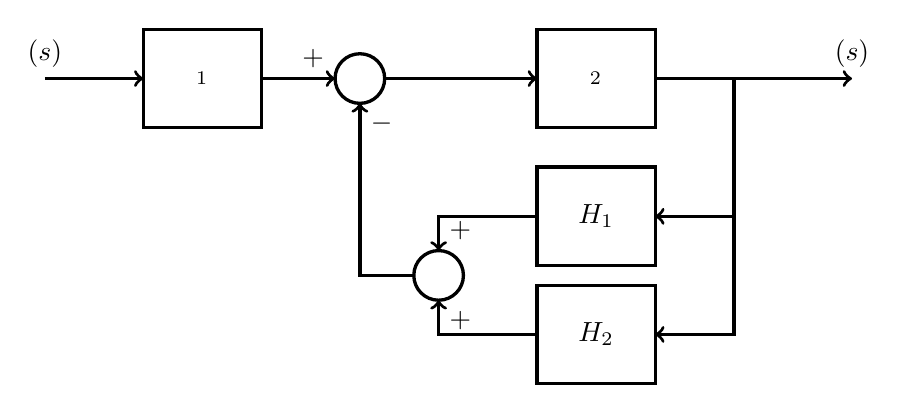
\begin{tikzpicture}[inner sep=0pt,outer sep=0pt,very thick,
sysblock/.style={draw,rectangle,inner sep=2pt,minimum width=1.5cm,minimum height=1.25cm,very thick}]
\draw (0,0) node[sysblock] (G1) {$\plant_{1}$};
\draw (2,0) node[draw,circle] (sum1) {$\rule{0pt}{18pt}$};
\draw (5,0) node[sysblock] (G2) {$\plant_{2}$};
\draw (G2.0) ++(1,0) node[fill=black] (a) {};

\draw (5,-1.75) node[sysblock] (H1) {$H_{1}$};
\draw (5,-3.25) node[sysblock] (H2) {$H_{2}$};
\draw (3,-2.5) node[draw,circle] (sum2) {$\rule{0pt}{18pt}$};

\draw[->] (-2,0) node[above=4pt] {$\inptLT(s)$} -- (G1.180);
\draw[->] (G1.0) -- (sum1.180) node[above left=4pt] {$+$};
\draw[->] (sum1.0) -- (G2.180);
\draw (G2.0) -- (a);
\draw[->] (a) -- ++(1.5,0) node[above=4pt] {$\outptLT(s)$};
\draw[->] (a) |- (H1.0);
\draw[->] (a) |- (H2.0);
\draw[->] (H1.180) -| (sum2.90) node[above right=4pt] {$+$};
\draw[->] (H2.180) -| (sum2.-90) node[below right=4pt] {$+$};
\draw[->] (sum2.180) -| (sum1.-90) node[below right=4pt] {$-$};

\end{tikzpicture}

\end{center}
\item Simplify the following block diagram using the ``untangling loops'' process found in the Appendix.
\begin{center}
\input{quizfigures/blockdiagramexample2.tex}
\end{center}

\end{enumerate}
\pagebreak

\subsection{Solutions}
\begin{enumerate}
\setlength{\itemsep}{5pt}
\setlength{\parskip}{0pt}
\setlength{\parsep}{0pt}
\item \rule{0pt}{12pt}\\
\begin{center}
\includegraphics[width=5in]{quizfigures/1soln}
\end{center}
\pagebreak
\item \rule{0pt}{12pt}\\
\begin{center}
\includegraphics[width=5in]{quizfigures/2asoln}\\
\includegraphics[width=5in]{quizfigures/2bsoln}
\end{center}
\end{enumerate}

\section{Resources}

\subsection{Books}
Block Diagrams are a fundamental tool in control systems, and is covered in introductory control systems textbooks.

\begin{itemize}
\item Norman S. Nise, {\em Control Systems Engineering}, Wiley
\begin{itemize}
\item 7th edition: Section 5.2
\end{itemize}
\item Richard C. Dorf and Robert H. Bishop, {\em Modern Control Systems}, Pearson
\begin{itemize}
\item 13th edition: Section 2.6
\end{itemize}
\item Gene F. Franklin, J. David Powell and Abbas Emami-Naeini,  {\em Feedback Control of Dynamic Systems}, Pearson
\begin{itemize}
\item 6th and 7th edition: Section 3.2
\end{itemize}
\end{itemize}


\subsection{Web resources}


\begin{itemize}
\item \url{https://www.youtube.com/watch?v=aMmthuU-4s4}: A 12 minute video covering the basic manipulations of block diagrams 
\end{itemize}

\section{Appendix}

\begin{frame}{Untangling Loops}
\begin{itemize}
	\item Sometimes, loops interfere with each other
\end{itemize}
\begin{center}
	\input{figures/blockdiagramexample2.tex}
\end{center}
\end{frame}

%\subsection{Example}
%
%\begin{frame}{Example 2}
%\begin{itemize}
%	\item Let's return to this example
%\end{itemize}
%\begin{center}
%	\input{figures/blockdiagramexample2.tex}
%\end{center}
%\end{frame}

By noting the rules for moving pickoff points around systems (blocks), we can obtain the equivalent diagram.
%\begin{frame}{Example 2:}{Equivalent Diagram}
\begin{center}
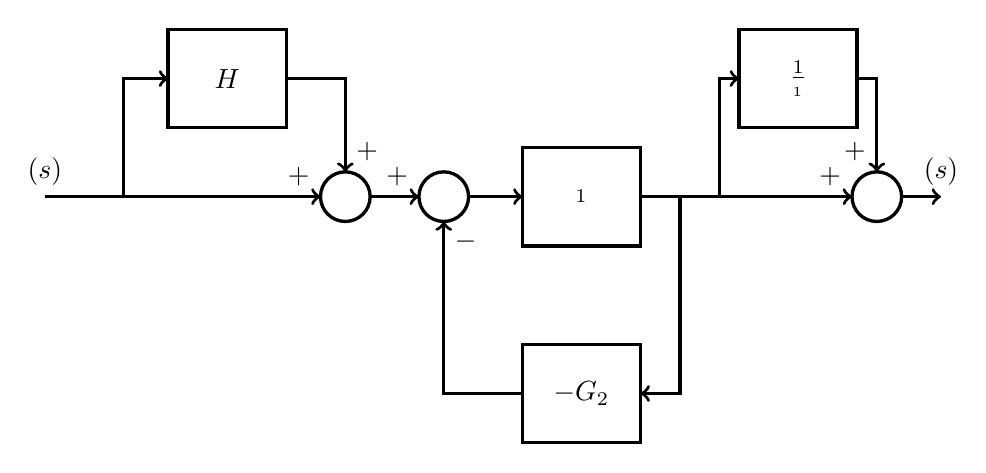
\begin{tikzpicture}[inner sep=0pt,outer sep=0pt,very thick,
sysblock/.style={draw,rectangle,inner sep=2pt,minimum width=1.5cm,minimum height=1.25cm,very thick}]
\draw (3.75,0) node[draw,circle] (sum1) {$\rule{0pt}{18pt}$};
\draw (2.5,0) node[draw,circle] (sum3) {$\rule{0pt}{18pt}$};
\draw (1,1.5) node[sysblock] (H) {$H$};
\draw (5.5,0) node[sysblock] (G1) {$\plant_{1}$};
\draw (G1.0) ++(.5,0) node[fill=black] (a) {};
\draw (G1.0) ++(1,0) node[fill=black] (b) {};
\draw (G1.0) ++(3,0) node[draw,circle] (sum2) {$\rule{0pt}{18pt}$};
\draw (G1.0) ++(2,1.5) node[sysblock] (GG) {$\frac{1}{\plant_{1}}$};

\draw (5.5,-2.5) node[sysblock] (G2) {$-G_{2}$};

\draw[->] (sum3.180) ++(-3.5,0) node[above=4pt] {$\inptLT(s)$} -- (sum3.180) node[above left=4pt] {$+$};
\draw[->] (sum3.180) ++(-2.5,0) |- (H.180);
\draw[->] (H.0) -| (sum3.90) node[above right=4pt] {$+$};
\draw[->] (sum3.0) -- (sum1.180) node[above left=4pt] {$+$};
\draw[->] (G1.0) -- (sum2.180) node[above left=4pt] {$+$};
\draw[->] (sum1.0) -- (G1.180);
\draw[->] (a) |- (G2.0);
\draw[->] (b) |- (GG.180);
\draw[->] (GG.0) -| (sum2.90) node[above left=4pt] {$+$};
\draw[->] (G2.180) -| (sum1.-90) node[below right=4pt] {$-$};
\draw[->] (sum2.0) -- ++(0.5,0) node[above=4pt] {$\outptLT(s)$};
\end{tikzpicture}

\end{center}
%\end{frame}

This diagram is easier to simplify using parallel and series rules. Note that a signal can be replaced by a signal-system combination in which the system is just a gain of 1, i.e., 

\begin{center}
\begin{tikzpicture}
\draw [-stealth](0,0) -- (4,0) node[above=4pt] {X(s)};
\end{tikzpicture}
\end{center}

is the same thing as 

\begin{center}
	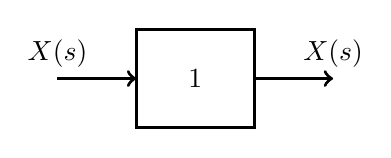
\begin{tikzpicture}[inner sep=0pt,outer sep=0pt,very thick,
sysblock/.style={draw,rectangle,inner sep=2pt,minimum width=1.5cm,minimum height=1.25cm,very thick}]
\draw (0,0) node[sysblock] (G) {$1$};
\draw[<-] (G.180) -- ++(-1,0) node[above=4pt] {$X(s)$};
\draw[->] (G.0) -- ++(1,0) node[above=4pt] {$X(s)$};
\end{tikzpicture}
\end{center}

The left and right parts of the example can therefore be combined as parallel combinations, while the middle one is a feedback loop, as shown below. These three blocks are now in series and can thus be multiplied to obtain the final transfer function. 
%\begin{frame}{Example 2:}{Simplified}
\begin{center}
\begin{tikzpicture}[inner sep=0pt,outer sep=0pt,very thick,
sysblock/.style={draw,rectangle,inner sep=2pt,minimum width=1.5cm,minimum height=1.25cm,very thick}]
\draw (0,0)  node[sysblock] (G1) {$H+1$};
\draw (2,0) node[sysblock]  (G2) {$\frac{\plant_{1}}{1-\plant_{2}\plant_{1}}$};
\draw (4,0)  node[sysblock] (G3) {$\frac{1}{\plant_{1}} +1$};
\draw[->] (G1.180) ++(-1.5,0) node[above=4pt] {$\inptLT(s)$} -- (G1.180);
\draw[->] (G1.0) -- (G2.180);
\draw[->] (G2.0) -- (G3.180);
\draw[->] (G3.0) -- ++(1.5,0) node[above=4pt] {$\outptLT(s)$};
\end{tikzpicture}

\end{center}
\[
\frac{\outptLT(s)}{\inptLT(s)} = \frac{(H+1)(G_{1}+1)}{1-G_{2}G_{1}}
\]
%\end{frame}


\end{document}